% $File: report.tex
% $Date: Sun Sep 01 11:01:17 2013 +0800
% $Author: wyx <ppwwyyxxc@gmail.com>

\documentclass[11pt,a4paper]{article}

\usepackage{fontspec,amsmath,amssymb,zhspacing,verbatim,minted,listings,zhmath}
\usepackage{titlesec, titletoc}
\usepackage{enumerate}
\usepackage[hyperfootnotes=false,colorlinks,linkcolor=blue,anchorcolor=blue,citecolor=blue]{hyperref}
\usepackage[backend=biber]{biblatex}
%\usepackage[dvips]{graphicx}
\usepackage{subfigure}
\usepackage{indentfirst}
\usepackage{float}			% don't automatically change location of figure [H]
\usepackage{chngpage}		% use \changetext to change page size
\usepackage{caption}\captionsetup{hypcap=true}  % ref to jump to object instead of caption
\newfontfamily\zhfont[BoldFont=SimHei,ItalicFont=KaiTi_GB2312]{SimSun}
\lstset{keywordstyle=\color{blue!70}, commentstyle=\color{red!50!green!50!blue!50},frame=shadowbox,rulesepcolor=\color{red!20!green!20!blue!20},
basicstyle=\footnotesize\ttfamily}
\zhspacing
\setlength{\parindent}{2em}

\usepackage{fancyhdr}
\changetext{}{2.2cm}{-1.1cm}{-1.1cm}{}
\pagestyle{fancy}
\setlength{\headheight}{15.2pt}
\lhead[]{}\rhead[]{}
\fancyhead[C]{\emph{Image Stitching}}


%use cell in tabular
\newcommand{\tabincell}[2]{\begin{tabular}{@{}#1@{}}#2\end{tabular}}

%thick shline
\newlength\savewidth
\newcommand\shline{\noalign{\global\savewidth\arrayrulewidth\global\arrayrulewidth 1pt}
                   \hline
                   \noalign{\global\arrayrulewidth\savewidth}}


%\renewcommand{\abstractname}{摘要}
%\renewcommand{\contentsname}{目录}
%\renewcommand{\tablename}{表}
%\renewcommand{\figurename}{图}
\defbibheading{bibliography}{\section{References}}
\bibliography{refs.bib}
\newcommand{\figref}[1]{\hyperref[fig:#1]{Fig\ref*{fig:#1}}}
\newcommand{\secref}[1]{\hyperref[sec:#1]{Sec \ref*{sec:#1}}}
\newcommand{\tabref}[1]{\hyperref[tab:#1]{Table \ref*{tab:#1}}}

% math function
\let\Oldsum\sum
\renewcommand{\sum}{\displaystyle\Oldsum}
\let\Oldprod\prod
\renewcommand{\prod}{\displaystyle\Oldprod}


% $File: mint-defs.tex
% $Date: Fri Jan 06 14:25:30 2012 +0800
% $Author: wyx <ppwwyyxxc@gmail.com>


% \inputmintedConfigured[additional minted options]{lang}{file path}{
\newcommand{\inputmintedConfigured}[3][]{\inputminted[fontsize=\footnotesize,
	label=#3,linenos,frame=lines,framesep=0.8em,tabsize=4,#1]{#2}{#3}}

% \phpsrc[additional minted options]{file path}: show highlighted php source
\newcommand{\phpsrc}[2][]{\inputmintedConfigured[#1]{php}{#2}}
% \phpsrcpart[additional minted options]{file path}{first line}{last line}: show part of highlighted php source
\newcommand{\phpsrcpart}[4][]{\phpsrc[firstline=#3,firstnumber=#3,lastline=#4,#1]{#2}}
% \phpsrceg{example id}
\newcommand{\phpeg}[1]{\inputminted[startinline,
	firstline=2,lastline=2]{php}{res/php-src-eg/#1.php}}

\newcommand{\txtsrc}[2][]{\inputmintedConfigured[#1]{text}{#2}}
\newcommand{\txtsrcpart}[4][]{\txtsrc[firstline=#3,firstnumber=#3,lastline=#4,#1]{#2}}

\newcommand{\pysrc}[2][]{\inputmintedConfigured[#1]{py}{#2}}
\newcommand{\pysrcpart}[4][]{\pysrc[firstline=#3,firstnumber=#3,lastline=#4,#1]{#2}}

\newcommand{\confsrc}[2][]{\inputmintedConfigured[#1]{squidconf}{#2}}
\newcommand{\confsrcpart}[4][]{\confsrc[firstline=#3,firstnumber=#3,lastline=#4,#1]{#2}}

\newcommand{\cppsrc}[2][]{\inputmintedConfigured[#1]{cpp}{#2}}
\newcommand{\cppsrcpart}[4][]{\cppsrc[firstline=#3,firstnumber=#3,lastline=#4,#1]{#2}}


\begin{document}
%\fontsize{10pt}{\baselineskip}
%\selectfont
%\maketitle

%\begin{abstract}

	%{\bf 关键词}
%\end{abstract}
% File: title.tex
% Date: Sat May 04 23:01:09 2013 +0800
% Author: Yuxin Wu <ppwwyyxxc@gmail.com>

\newcommand{\HUGE}{\fontsize{29pt}{29pt}\selectfont}
\renewcommand{\today}{\number\year 年 \number\month 月 \number\day 日}
\begin{titlepage}

% 首行的位置往上调整。但vspace前面需要有东西才会起效。

\phantom{Start!}

\vspace{-1.7cm}

\begin{flushleft}

\emph{\Large Dept. of CST, Tsinghua University}\\[0.2cm]

\emph{\Large Digital Image Processing}\\[5.2cm]

% Title

\hspace{3cm}{ \HUGE \bfseries Image Stitching}\\[0.4cm]


\hspace{3cm} {\huge \bfseries Project Report}

\end{flushleft}





\vfill



\begin{flushright}

{

%\setCJKmainfont{Adobe Kaiti Std}

% \pillar:使用一种统一的方法提高行高

\newcommand{\pillar}{ {\Huge \phantom{A}} }

\large

\begin{tabular}{lc}

\pillar Name & Yuxin Wu\\\cline{2-2}

\pillar Student No.& 2011011271 \\\cline{2-2}

\pillar Class  & CST-14 \\\cline{2-2}

\pillar Mail &ppwwyyxxc@gmail.com \\\cline{2-2}

\end{tabular}

}

\end{flushright}

\end{titlepage}

\tableofcontents
%\newpage

%\titleformat*{\section}{\centering\Large\bf}
% File: intro.tex
% Date: Sat May 04 22:49:57 2013 +0800
% Author: Yuxin Wu <ppwwyyxxc@gmail.com>
\section{Usage}
\subsection{Compilation}
Dependencies:

\begin{enumerate}
    \item gcc >= 4.7
    \item GNU make
    \item Magick++
    \item boost MTL (Matrix Template Library) installed in /usr/include/boost/numeric/.
      It can be downloaded from \url{http://www.simunova.com/node/145}. A copy is attached in the submitted package.
\end{enumerate}

Compilation:
\begin{lstlisting}
$ make
\end{lstlisting}

\subsection{Run}
Various parameters are saved in \verb|src/config.cfg|.
Without special needs, we only have to modify \verb|PANO, TRANS, CROP|.

The program does some extra work to beautify the output
if knowing the input pictures were taken by a camera
moving in pure translation or pure rotation.

\verb|PANO = 1| tells that the camera moved in pure rotation. A panorama is expected to be the output;

\verb|TRANS = 1| tells that the camera moved in pure translation. Result will be better than the one with \verb|TRANS| unset;

\verb|CROP| decides whether to crop the final image to a rectangular;

Use \verb|./main <file1> <file2> <file3> ...| in the command line to run the program.
Output file is \verb|out.png|.

Usually, input images should not exeeds $20(files)\times 1500(pixels) \times 1000(pixels)$, since your computer may not have enough memory.

The input file names given in the command line need to be well ordered.

\subsection{Examples}
\begin{enumerate}
\item TRANS = 1
  \begin{lstlisting}
$ ./main ../data/flower/small*
  \end{lstlisting}
\begin{figure}[H]
  \centering
  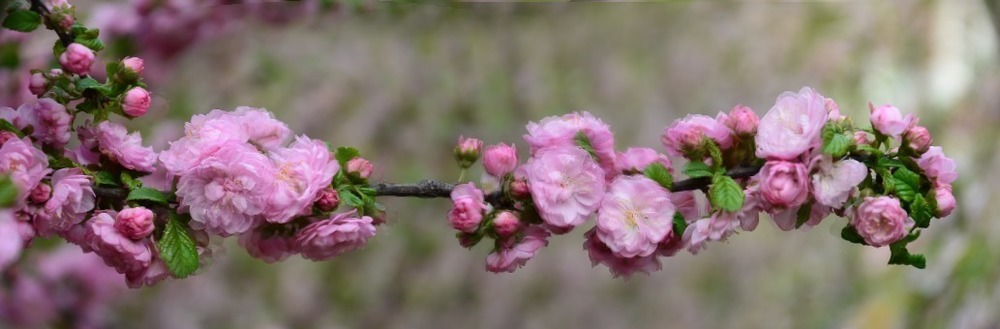
\includegraphics[scale=0.27]{res/small.png}
\end{figure}


  \item PANO = 1
    \begin{lstlisting}
$ ./main ../data/ground/small*
    \end{lstlisting}
    The result is shown in \figref{cropped}.
\end{enumerate}

% File: algo.tex
% Date: Sun May 05 17:04:00 2013 +0800
% Author: Yuxin Wu <ppwwyyxxc@gmail.com>

\section{Algorithms}
\subsection{Feature Detection}
Lowe's SIFT algorithm\cite{sift} is implemented.

The algorithm follows the following procedure:
\begin{enumerate}
  \item Build a Scale-Space, which consists of $ S \times O$ grey images.
    The original image is resized in $ O$ different sizes (octaves), and each is then Gaussian-Blured
    by $ S$ different $ \sigma$s.
    \begin{figure}[H]
      \centering
      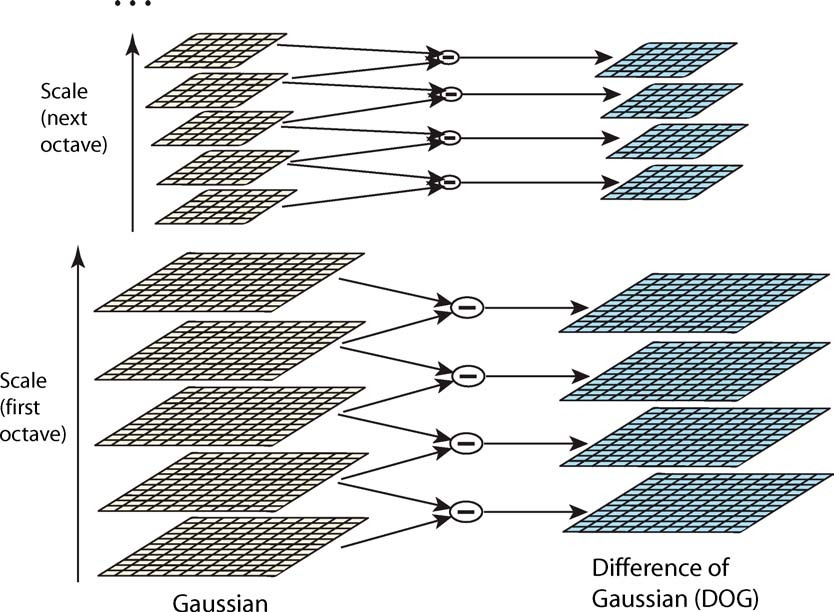
\includegraphics[scale=0.35]{res/dog.png}
      \caption{Scale Space and DOG Space \label{fig:dog}}
    \end{figure}

  \item Build a Difference-of-Gaussian Space.
    In each octave, calculate the differences of every two adjacent blured images.
    Therefore, DOG Space consists of $ (S - 1) \times O$ grey images.
    As shown in \figref{dog}.

  \item Detect extrema. In DOG Space, detect all the minimum and maximum
    by comparing a pixel with its 26 neighbors in three directions: $ x, y, \sigma$.
    See \figref{extrema} and \figref{extrema2}
    \begin{figure}[H]
      \begin{minipage}[b]{0.46\linewidth}
        \centering
        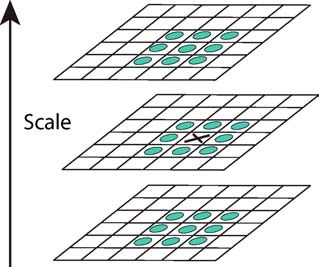
\includegraphics[scale=0.4]{res/extrema.png}
        \caption{Extrema Detection\label{fig:extrema}}
      \end{minipage}
      \hspace{1em}
      \begin{minipage}[b]{0.46\linewidth}
        \centering
        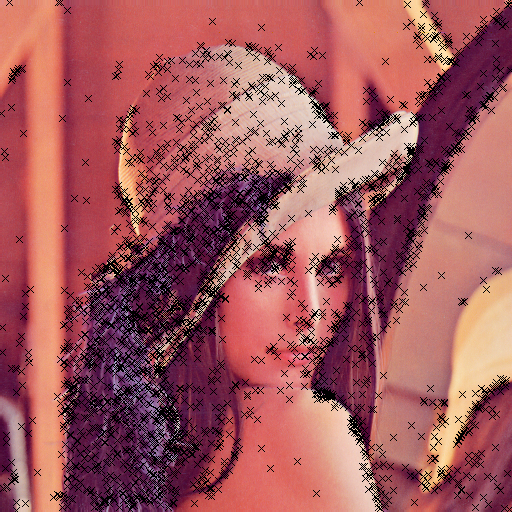
\includegraphics[scale=0.35]{res/extrema_lenna.png}
        \caption{Extrema Example\label{fig:extrema2}}
      \end{minipage}
    \end{figure}

  \item Keypoint Localization.
    Use linear interpolation to calculate offset,
    moving the extrema to a more accurate location.
    Then reject the points with low contrast or on the edge to get distinctive features.
    See \figref{feature1}, \figref{feature2}, \figref{feature3}.
    \begin{figure}[H]
      \begin{minipage}[b]{0.46\linewidth}
        \centering
        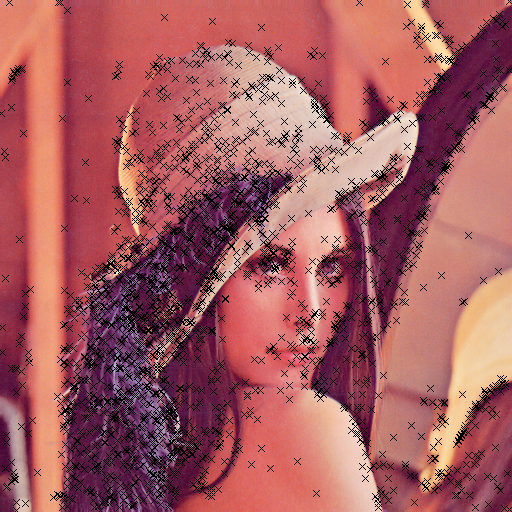
\includegraphics[scale=0.4]{res/feature_after_offset.png}
        \caption{After Localization \label{fig:feature1}}
      \end{minipage}
      \hspace{1em}
      \begin{minipage}[b]{0.46\linewidth}
        \centering
        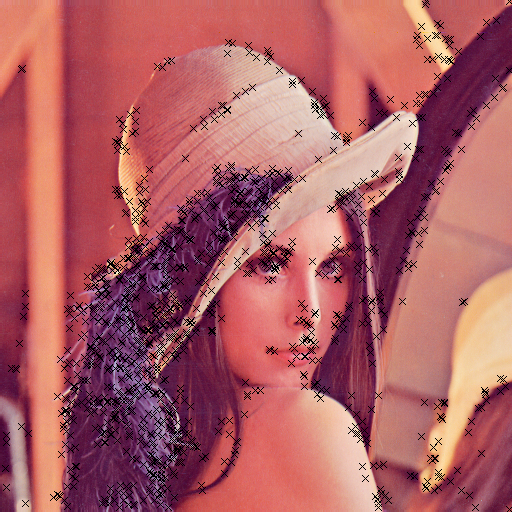
\includegraphics[scale=0.4]{res/feature_after_contrast.png}
        \caption{After Rejecting Low Contrast\label{fig:feature2}}
      \end{minipage}

      \begin{minipage}[b]{0.46\linewidth}
        \centering
        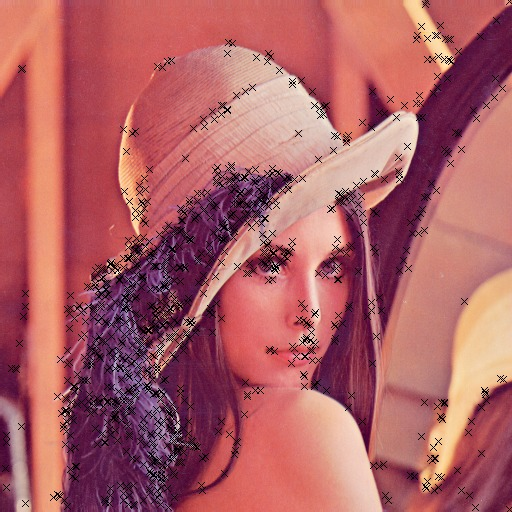
\includegraphics[scale=0.4]{res/feature_point.png}
        \caption{After Eliminating Edge Point\label{fig:feature3}}
      \end{minipage}
      \hspace{1em}
      \begin{minipage}[b]{0.46\linewidth}
        \centering
        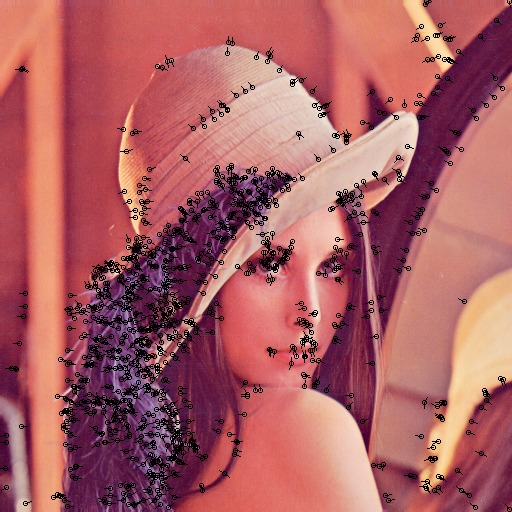
\includegraphics[scale=0.4]{res/feature_dir.png}
        \caption{After Assigning Orientation\label{fig:feature4}}
      \end{minipage}
    \end{figure}

  \item Orientation Assignment.
    We have to first calculated the gradient and orientation of every point in the Scale Space.
    For each keypoint, a histogram of the orientations of its nearby points is built,
    weighted by a gaussian kernel and the magnitude of gradient.
    The peak in the histogram is chosen to be the orientation of the keypoint, as shown by the arrow in \figref{feature4}.

  \item Descriptor Representation.
    Lowe suggested choosing 16 points around the keypoint and building 16 orientation histograms,
    each with 8 different possible values.
    Since all the orientation is relative to the keypoint's orientation,
    this feature is roatation-invariant. The final SIFT feature is a 128-dimensional array.

  \item Feature Matching.
    The Euclidean distance of the 128-dimensional descriptor is the criteria for feature matching between two images.
    A match is considered not convincing and therefore rejected
    if the distances to its closest neighbor and second-closest neighbor are similar.
    The result is shown in \figref{match}.
    \begin{figure}[H]
      \centering
      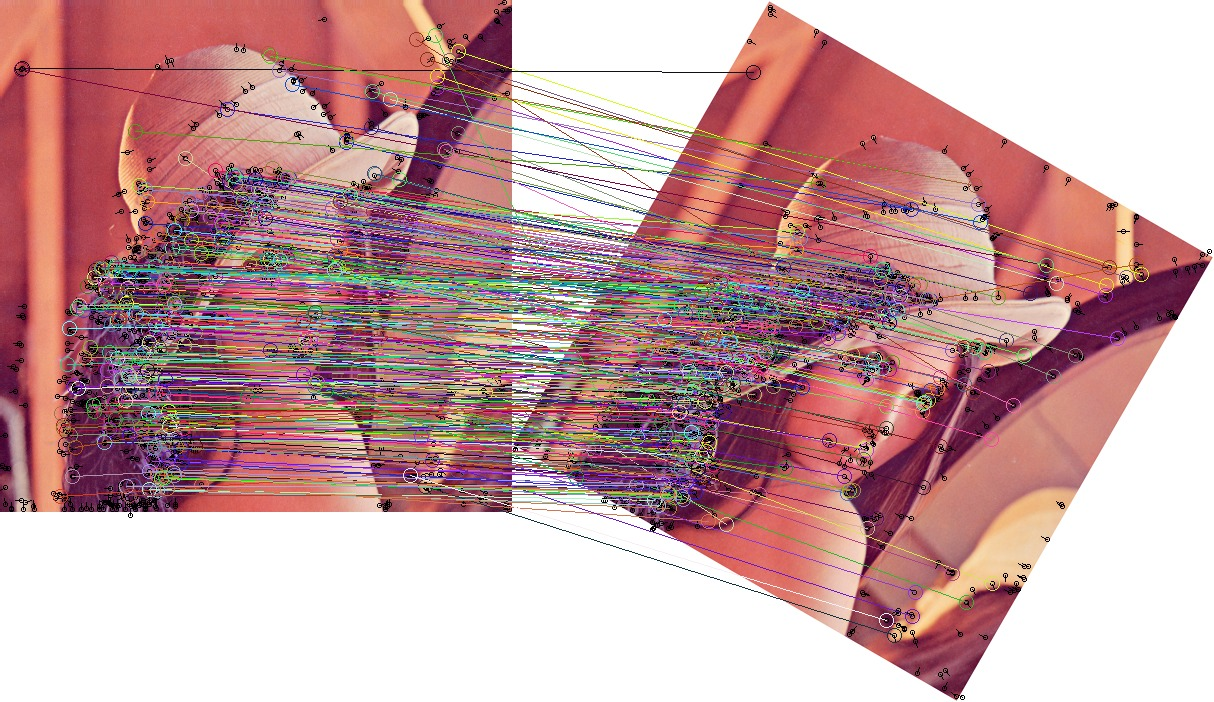
\includegraphics[width=\textwidth]{res/match.png}
      \caption{Matching Result\label{fig:match}}
    \end{figure}


    \subsection{Warping}
    A homography transform is needed to match the keypoints.
    But a pure homography transform on a planar works
    only if the camera moved in pure translation or toward a fixed center.

    If a rotational input is given, using homography on a planar leads to vertical distortion, like \figref{distort}.
    \begin{figure}[H]
      \centering
      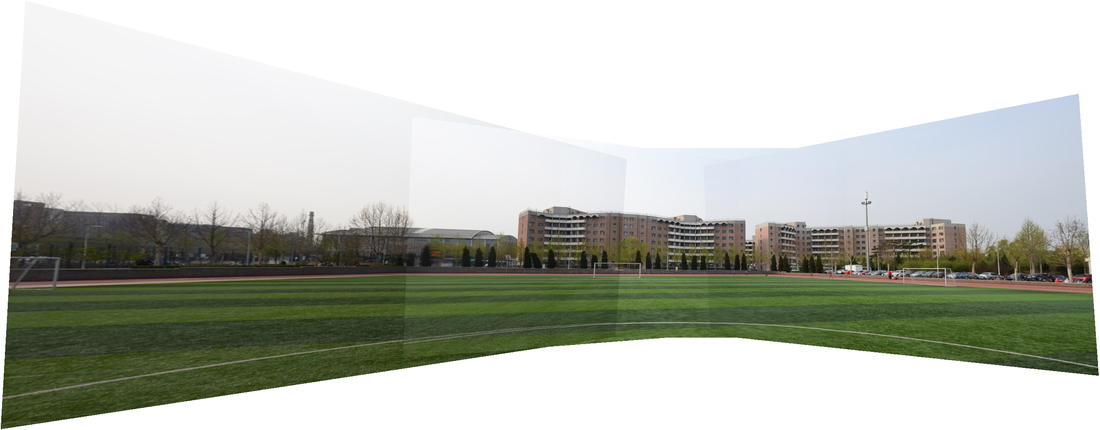
\includegraphics[width=\textwidth]{res/distort.png}
      \caption{Vertical Distortion with Homography on a Planar\label{fig:distort}}
    \end{figure}

    Therefore, if the option \verb|TRANS = 0|,
    every input image will be projected to a cylinder by the following formula:

    \[  \begin{cases}
        x' = k\arccos{\dfrac{x}{\sqrt{x^2 + z^2}}}\\
        y' = k\dfrac{y}{\sqrt{x^2 + z^2}}
      \end{cases}\]
    where $ z$ is chosen to be $ \max\{width, height\}$.  The result is in shown in \figref{cyl}.
    \begin{figure}[H]
      \centering
      \begin{minipage}[b]{0.24\linewidth}
        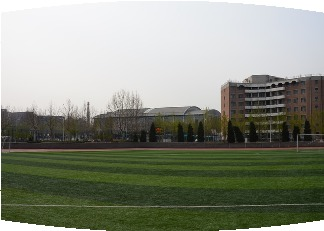
\includegraphics[scale=0.3]{res/1.png}
      \end{minipage}
      \begin{minipage}[b]{0.24\linewidth}
        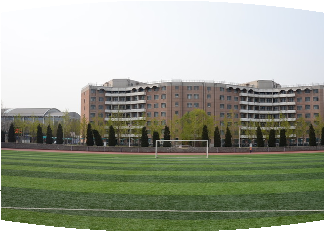
\includegraphics[scale=0.3]{res/2.png}
      \end{minipage}
      \begin{minipage}[b]{0.24\linewidth}
        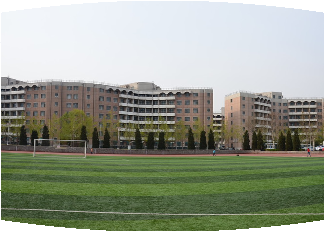
\includegraphics[scale=0.3]{res/3.png}
      \end{minipage}
      \begin{minipage}[b]{0.24\linewidth}
        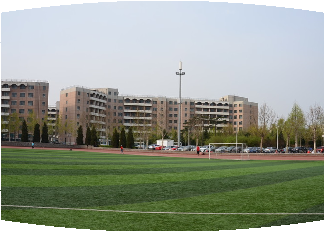
\includegraphics[scale=0.3]{res/4.png}
      \end{minipage}

      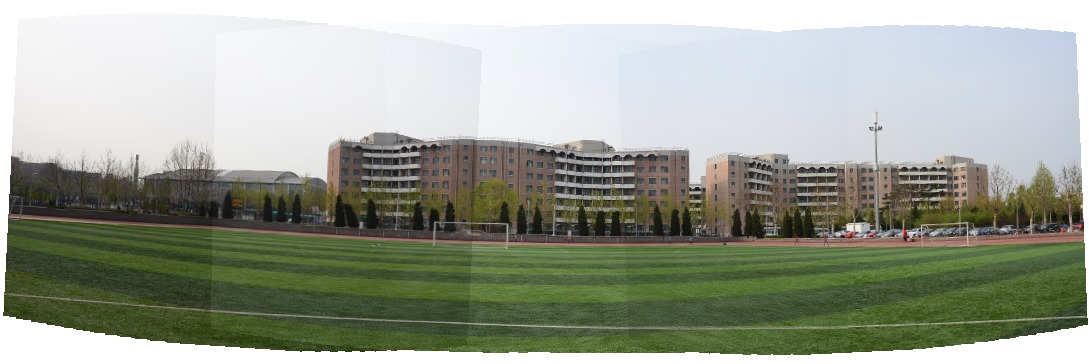
\includegraphics[width=\textwidth]{res/warped_stitch.png}
      \caption{Stitching Result After Projection\label{fig:cyl}}
    \end{figure}

\end{enumerate}

\subsection{Transformation}
RANSAC (Random Sample Consensus) algorithm\cite{ransac} is used to calculate a transformation matrix.
In every iteration, several matched pairs is randomly chosen to calculate a best-fit transformation matrix,
and the number of pairs it fits within all the data is calculated.

I tried three kinds of transformation:
\begin{enumerate}
  \item Homography One: $H = \begin{bmatrix} a_{11} &a_{12} & a_{13}\\ a_{21} & a_{22} & a_{23}\\ a_{31} & a_{32} & 1\end{bmatrix}$

  \item Homography Two:
    $H = \begin{bmatrix} a_{11} &a_{12} & a_{13}\\ a_{21} & a_{22} & a_{23}\\ a_{31} & a_{32} & a_{33}\end{bmatrix} $
    and $\begin{Vmatrix} H \end{Vmatrix} = 1$

  \item Affine:
    $A = \begin{bmatrix} a_{11} &a_{12} & a_{13}\\ a_{21} & a_{22} & a_{23}\\ 0 & 0 & 1\end{bmatrix}$
\end{enumerate}

Given a set of matches, affine and the first kind of homography transformation can be solved
by least-squares fitting an over-determined linear system.
The second kind of homography transformation can be solved by singular value decomposition.
The two homography lead to similar results, which are used when \verb|TRANS = 1|.
For warped images, all the transformation work well.
In this project, affine transformation is used for generating panoramas.

\subsection{Straightening}
\begin{figure}[H]
  \centering
  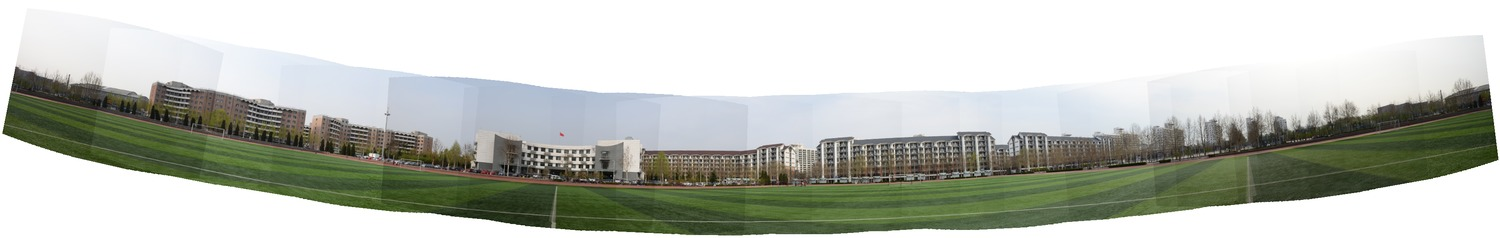
\includegraphics[width=\textwidth]{res/bend.png}
  \caption{Bended Panorama\label{fig:bend}}
\end{figure}

Since the tilt of camera is unknown, the output panorama might be bended as shown in \figref{bend}.
Instead of using the first image as the pivot, and calculating all the other transformation relative to it,
using the image in the middle as the pivot can help reduce the tilt effect.
Moreover, when the option \verb|PANO = 1| is set, an automatic straightening process will be executed.

First, a binary search on the tilt factor is performed, aiming to make the result ``longer''.
Second, the program will try to catenate the first image after the last one,
and then do a global rotation to ensure that the head and tail are aligned horizontally.
After this two processes, the result is like \figref{unbend}.

\begin{figure}[H]
  \centering
  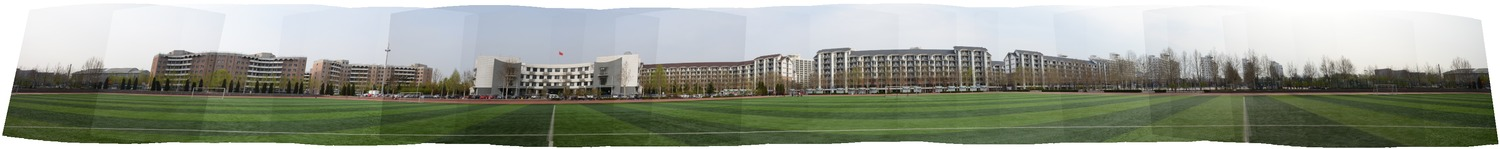
\includegraphics[width=\textwidth]{res/unbend.png}
  \caption{Straightened Panorama\label{fig:unbend}}
\end{figure}

\subsection{Blending}
The size of the final result is determined immediately after calculating all the transformations.
And the pixel value in the result image is calculated by an inverse transformation and interpolation with nearby pixels,
in order to reduce alias effect.

As for the overlap effect, the distance of the pixel to each image center is used to calculate a weighted sum of the pixel value.
The result is almost seamless, as shown in \figref{blend}.
\begin{figure}[H]
  \centering
  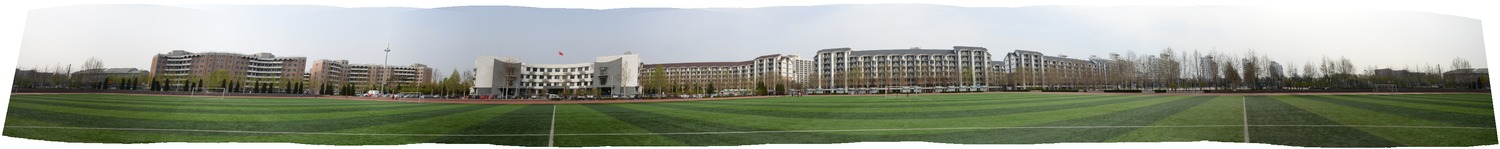
\includegraphics[width=\textwidth]{res/blend.png}
  \caption{Blended Result\label{fig:blend}}
\end{figure}

\subsection{Cropping}
When the option \verb|CROP = 1| is set,
the program simply manage to find a rectangular with largest area within the original irregular result.

A classic $ O(n \times m)$ algorithm is used, where $ n, m$ is the height and width of the original result.

For each row $i$, update
\begin{flalign*}
 h[j] &= \begin{cases}0,& if\ i = 0\ or\ A[i][j]\ is\ outside \\ h[j] + 1,& otherwise\end{cases}\\
 r[j] &= \max\{ k \in [0, m) \cap \mathbf{N}: h[t] \ge h[j], \forall j \le t \le k\} \\
l[j]  &= \min\{ k \in [0, m) \cap \mathbf{N} : h[t] \ge h[j], \forall k \le t \le j\}\\
\end{flalign*} for every $ j \in [0, n) $ in amortized $ O(1)$ time, and the corresponding area is $ (r[j] - l[j] + 1) \times h[j]$.

The cropped final result is shown in \figref{cropped}
\begin{figure}[H]
  \centering
  \includegraphics[width=\textwidth]{res/results/ground.png}
  \caption{Cropped Result\label{fig:cropped}}
\end{figure}


% File: result.tex
% Date: Sun Dec 29 00:10:41 2013 +0800
% Author: Yuxin Wu <ppwwyyxxc@gmail.com>

\section{More Results}
\begin{figure}[H]
  \centering
  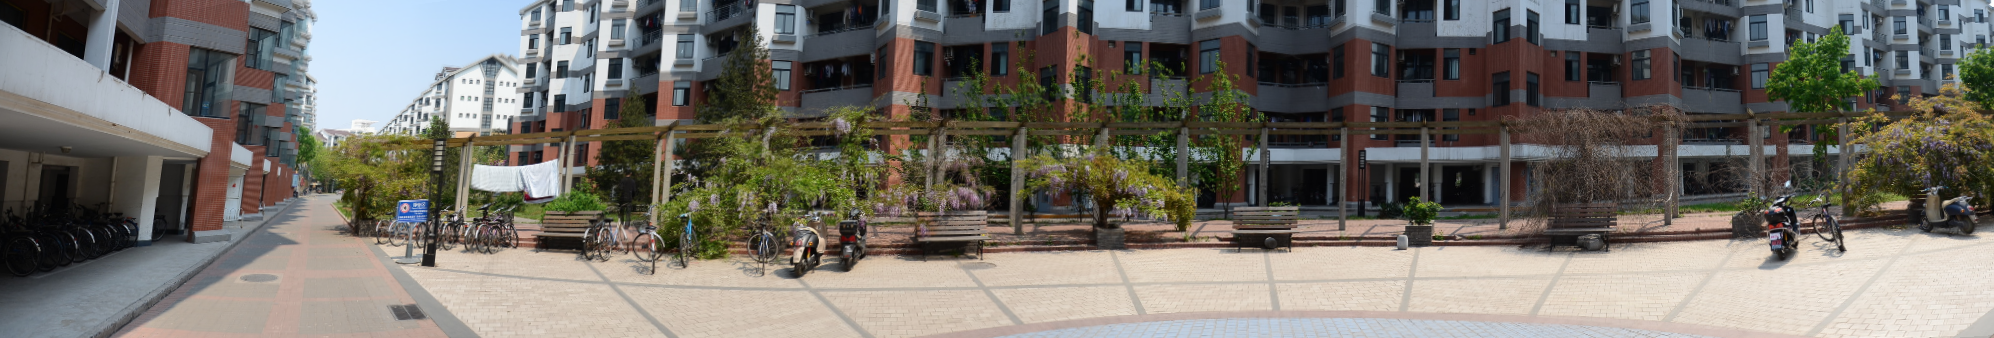
\includegraphics[width=\textwidth]{res/results/apartment.png}
\end{figure}
\begin{figure}[H]
  \centering
  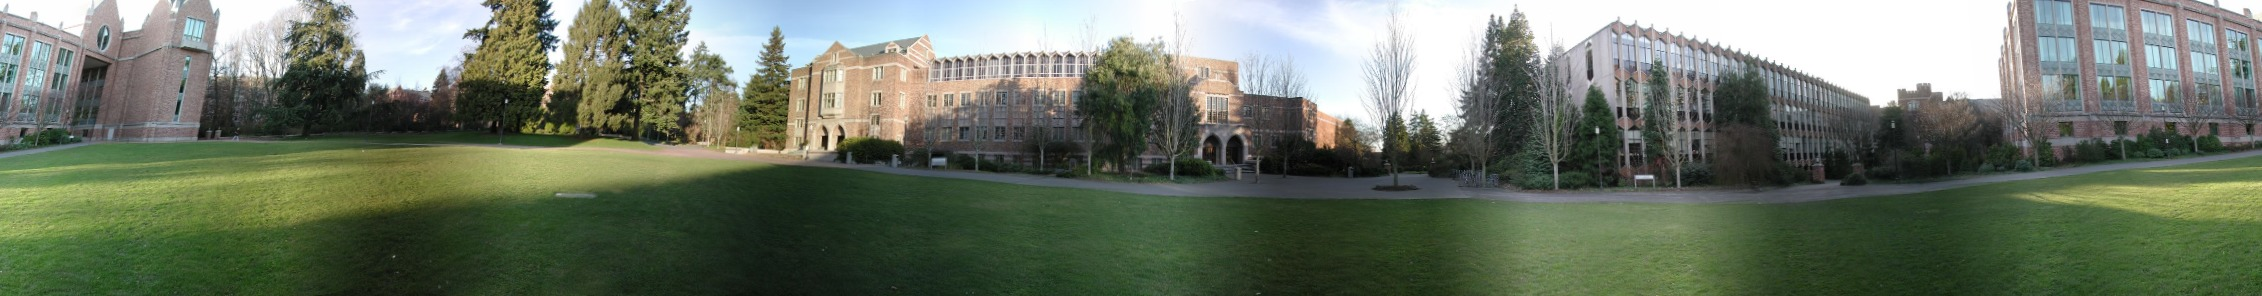
\includegraphics[width=\textwidth]{res/results/campus.png}
\end{figure}

\begin{figure}[H]
  \centering
  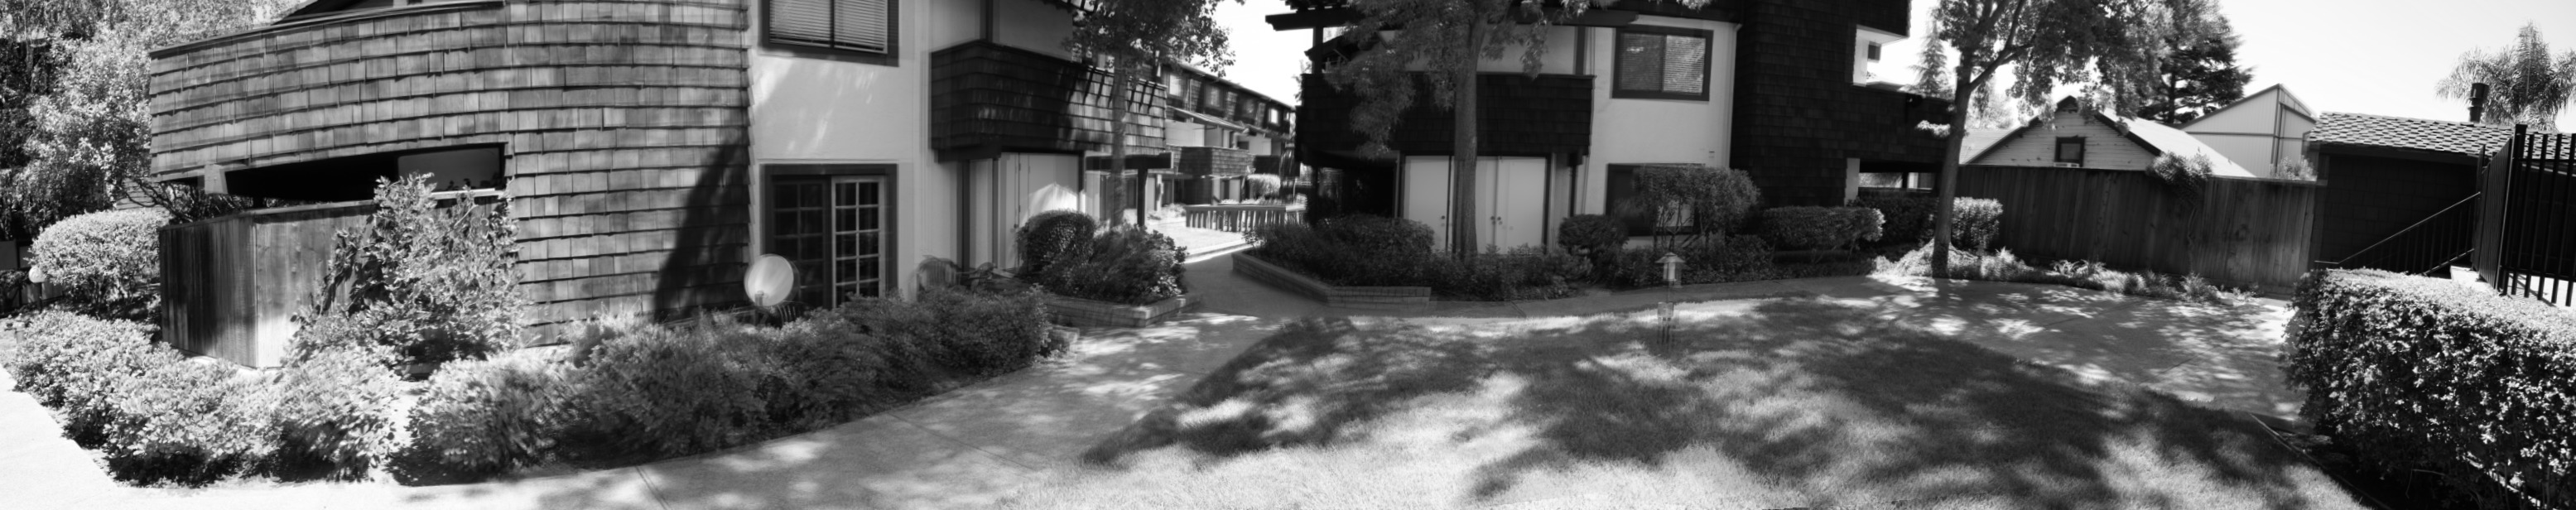
\includegraphics[width=\textwidth]{res/results/yard.png}
\end{figure}

%\begin{figure}[H]
  %\centering
  %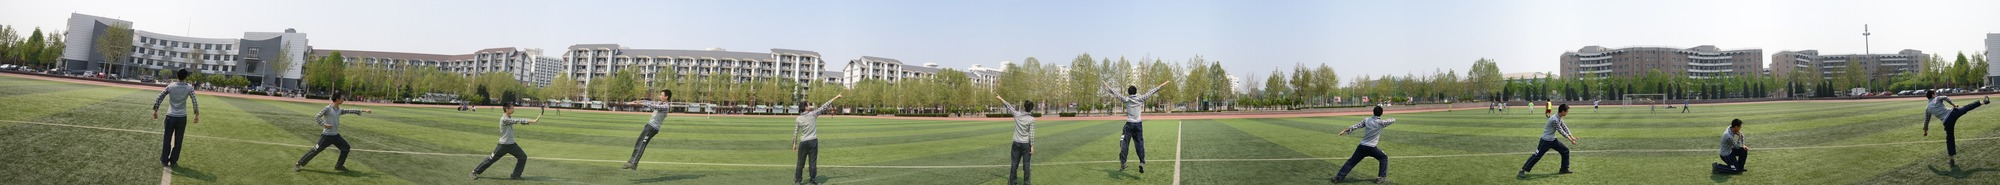
\includegraphics[width=\textwidth]{res/results/myself.png}
%\end{figure}

%\begin{figure}[H]
  %\centering
  %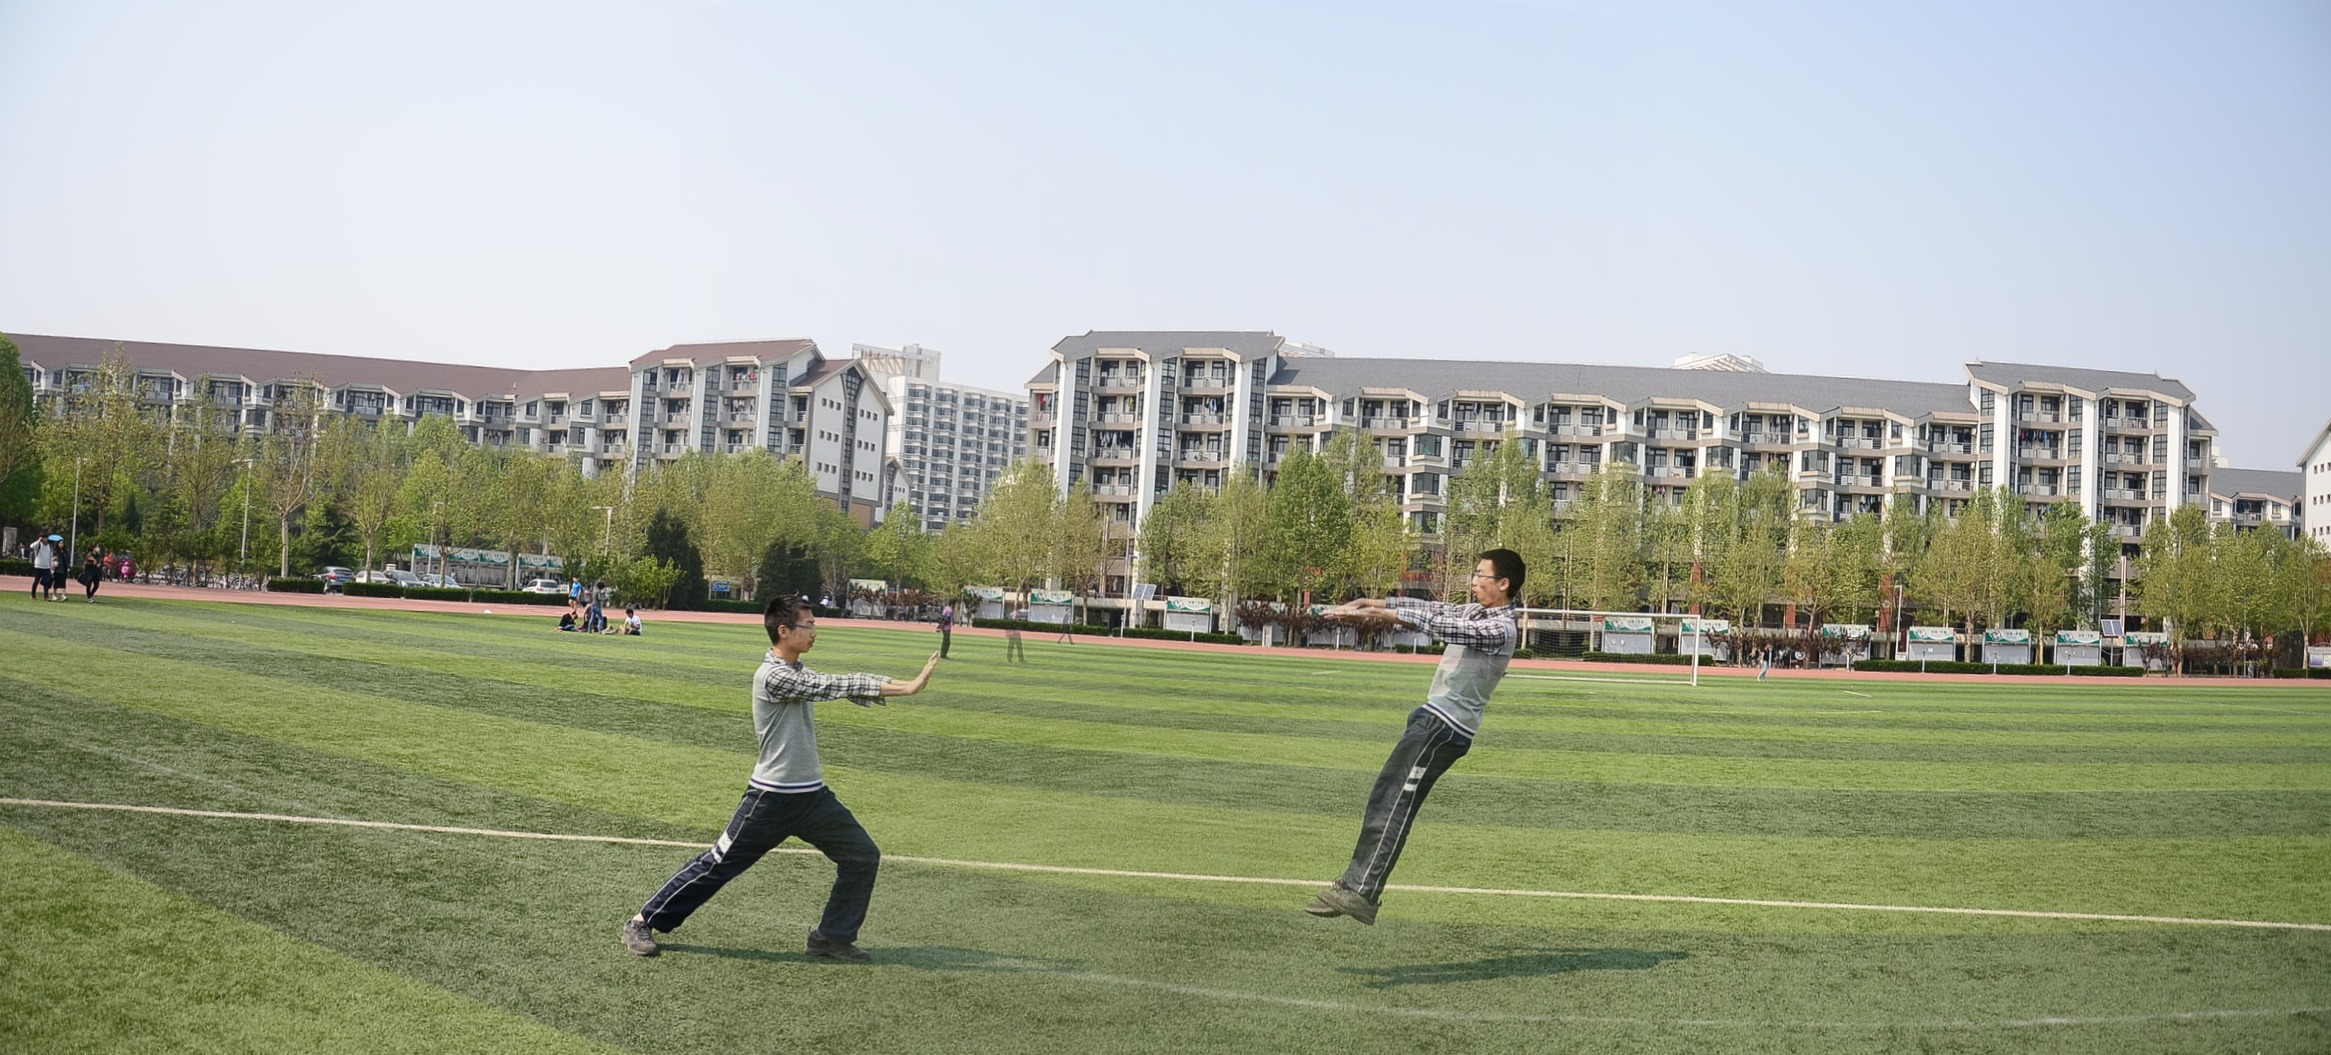
\includegraphics[width=\textwidth]{res/results/fight.png}
%\end{figure}

\newpage
By adding a polar transformation, we can simply turn the panorama into this:

\begin{figure}[H]
  \centering
  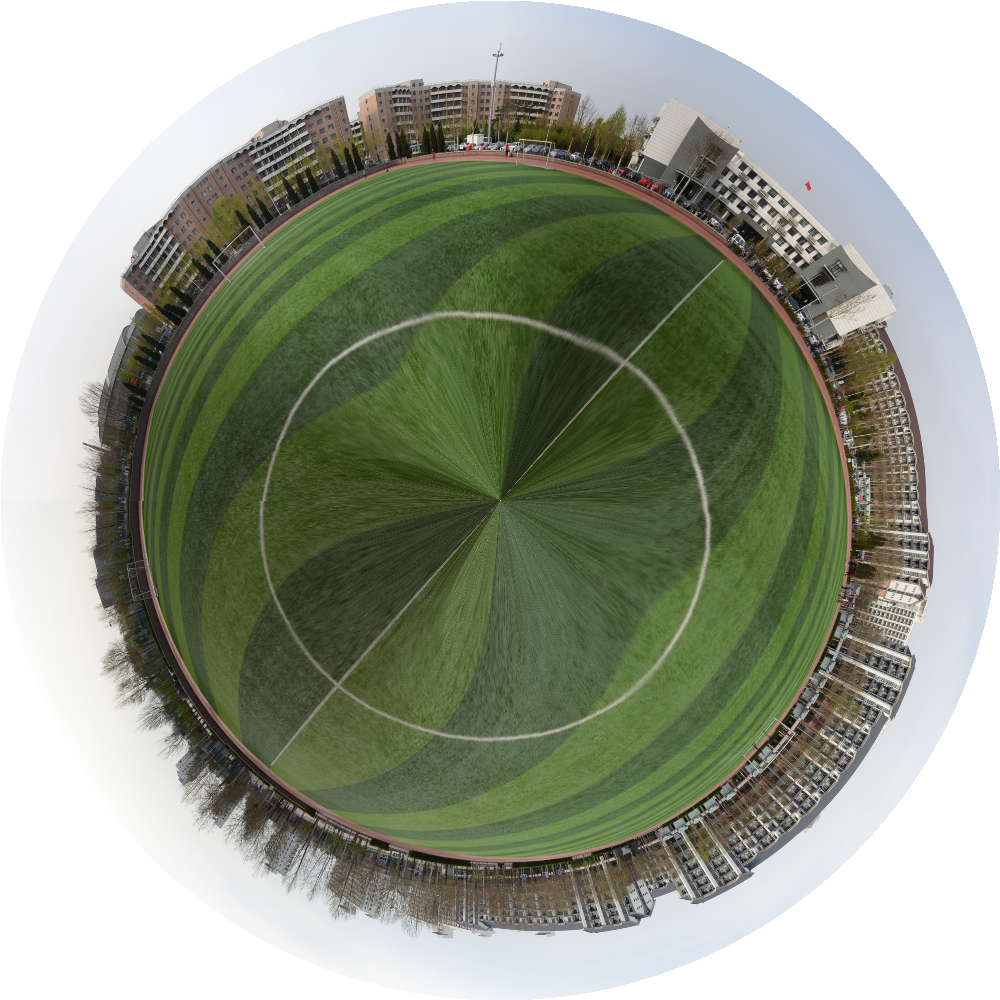
\includegraphics[width=\textwidth]{res/results/planet.png}
\end{figure}

\printbibliography

\end{document}

